%-------------------------------------------------------------------------
%
% Latex-Beamer theme for non-commercial/private use
%
% Author: Xian Qiu
% Date: May 1, 2015
% Version: 1.1beta
%
% ------------------------------------------------------------------------



%-------------------------------------------------------------------------
% Chapterframe
%-------------------------------------------------------------------------

\newenvironment{chapterframe}
{
	\setbeamertemplate{frametitle}[chaptertitle]
	\setbeamertemplate{itemize item}[tts@square]
    \begin{frame}
    	\begin{minipage}{0.15\paperwidth} % expression "\paperwidth/5" is not allowed
    		\tikz\path (0,0) -- (0.15*\paperwidth,0.15*\paperwidth);
    	\end{minipage}\hfill\minipage{0.6\paperwidth}

}{  
    \endminipage
    \end{frame}
}


%-------------------------------------------------------------------------
% Thanksframe
%-------------------------------------------------------------------------

\newenvironment{thanksframe}
{
	\setbeamertemplate{frametitle}[chaptertitle]
	\begin{frame}[plain]
		\begin{minipage}{0.15\paperwidth} % expression "\paperwidth/5" is not allowed
			\tikz\path (0, 0) -- (0.15*\paperwidth,0.15*\paperwidth);
		\end{minipage}\hfill\minipage{0.55\paperwidth}
		
	}{  
		%  Tutte's 8-cage
		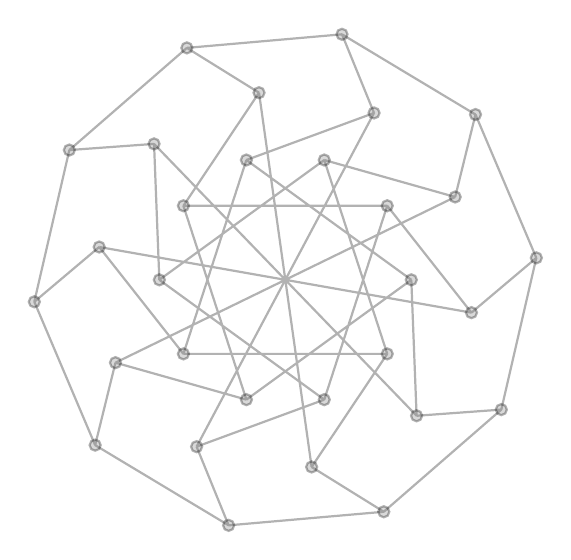
\begin{tikzpicture}[opacity=0.3, thick, scale=0.8]
		\tikzstyle{every node}=[circle, draw, fill=black!50,
		inner sep=0pt, minimum width=4pt]
		\draw \foreach \x in {0,36,...,324}
		{
			(\x:2) node {}  -- (\x+108:2)
			(\x-10:3) node {} -- (\x+5:4)
			(\x-10:3) -- (\x+36:2)
			(\x-10:3) --(\x+170:3)
			(\x+5:4) node {} -- (\x+41:4)
		};
		\end{tikzpicture}
		\endminipage
	\end{frame}
}